\chapter{Registri}

\section{Contatori}
Un contatore è un registro usato per contare il numero di occorrenze di un determinato evento.
Tipicamente, gli eventi che può contare sono i colpi di clock o le occorrenze di alcuni valori (o sequenze) di input. 

\subsubsection{Contatore modulo 8}
Il contatore modulo 8 parte da 0 e ad ogni fronte d'onda discendente del clock incrementa di 1 il suo valore, fino ad arrivare a 7; poi torna a 0 e ricomincia.
\begin{figure}[ht]
    \centering
    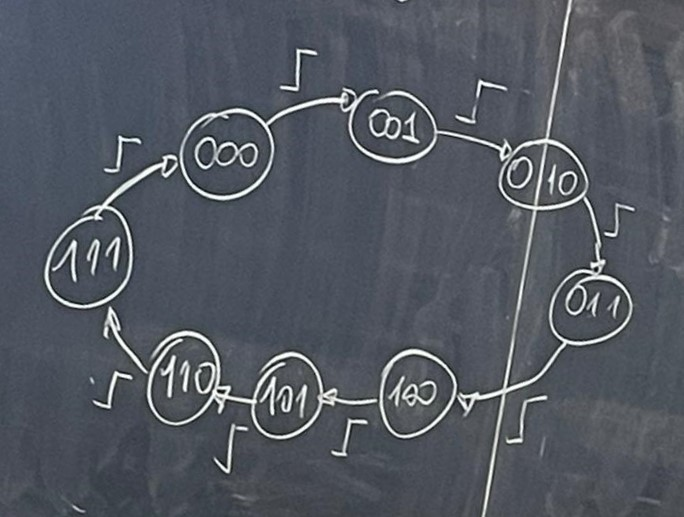
\includegraphics[width = 8cm]{images/contatori.jpeg}
    \caption{Automa contatore modulo 8}
    \label{fig:contatore_mod_8}
\end{figure}

Troviamo le equazioni di $j$ e $k$ con le k-mappe:
\begin{center}
$j_0$ = 
\begin{tabular}{|c|c|c|c|c|}
    \hline \diagbox[width=1.5cm]{$y_2$}{$y_1y_0$} & 00 & 01 & 11 & 10 \\\hline\hline
    0 & 0 & 1 & - & -\\\hline
    1 & 0 & 1 & - & -\\\hline
\end{tabular}\hspace{1cm}
$j_1$ =
\begin{tabular}{|c|c|c|c|c|}
    \hline \diagbox[width=1.5cm]{$y_2$}{$y_1y_0$} & 00 & 01 & 11 & 10 \\\hline\hline
    0 & - & - & 1 & 0\\\hline
    1 & - & - & 1 & 0\\\hline
\end{tabular}\hspace{1cm}
$j_2$ = 
\begin{tabular}{|c|c|c|c|c|}
    \hline \diagbox[width=1.5cm]{$y_2$}{$y_1y_0$} & 00 & 01 & 11 & 10 \\\hline\hline
    0 & 0 & 0 & 1 & 0\\\hline
    1 & - & - & - & -\\\hline
\end{tabular} 
\end{center}

Otteniamo così le equazioni:
\begin{equation*}
    J_0 = K_0 = 1\hspace{0,5cm}J_1 = K_1 = y_0\hspace{0,5cm}J_2 = K_2 = y_1y_0
\end{equation*}

Con la tavole degli stati futuri otteniamo:
\begin{table}[ht]
    \centering
    \begin{tabular}{|c|c|c|}
         \hline $y_2 y_1 y_0$ & $Y_2 Y_1 Y_0$ & $J_2 K_2 J_1 K_1 J_0 K_0$\\\hline\hline
        0 0 0 & 0 0 1 & 0 - 0 - 1 -\\\hline
        0 0 1& 0 1 0& 0 - 1 - - 1\\\hline
        0 1 0& 0 1 1& 0 - - 0 1 -\\\hline
        0 1 1& 1 0 0& 1 - - 1 - 1\\\hline
        1 0 0& 1 0 1& - 0 0 - 1 -\\\hline
        1 0 1& 1 1 0& - 0 1 - - 1\\\hline
        1 1 0& 1 1 1& - 0 - 0 1 -\\\hline
        1 1 1& 0 0 0& - 1 - 1 - 1\\\hline
    \end{tabular}
\end{table}

Avendo il contatore modulo $2^3$ posso rappresentarlo con 3 flip-flop:
\begin{figure}[H]
    \centering
    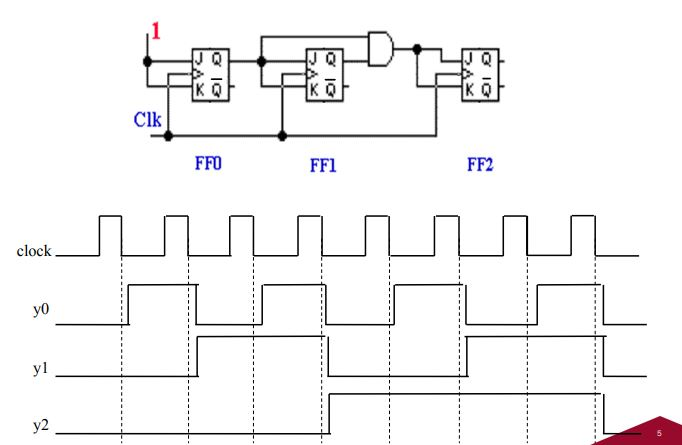
\includegraphics[width = 10cm]{images/contatore_mod_8.JPG}
    \caption{Contatore modulo 8 con 3 flip-flop}
\end{figure}

\subsubsection{Contatore bidirezionale}
Il contatore bidirezionale è un particolare tipo di contatore che, come suggerisce il termine, può contare crescendo o decrescendo.

\begin{figure}[ht]
    \centering
    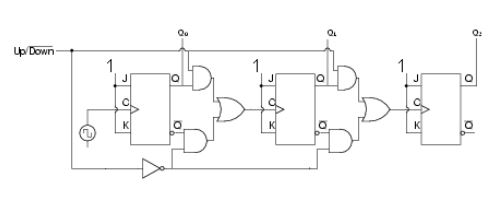
\includegraphics[width = 12cm]{images/contatore_bidirezionale.JPG}
    \caption{Contatore bidirezionale}
    \label{fig:contatore_bidirezionale}
\end{figure}

Se come line di controllo (c) si ottiene 1, il contatore conterà in avanti, in caso contrario, con 0 conta indietro.

\subsubsection{Contatore modulo k}
Spesso, i flip-flop sono equipaggiati con due ulteriori ingressi, chiamati PRESET e CLEAR, che funzionano in maniera asincrona rispetto al clock: essi cioè sono usati per settare o resettare il flip-flop in modo istantaneo, cioè indipendentemente dalle entrate e dal clock.

\begin{figure}[ht]
    \centering
    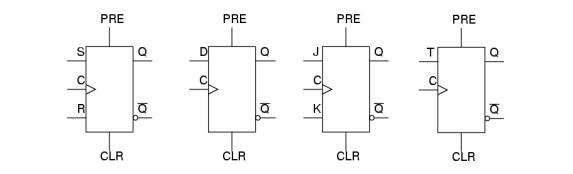
\includegraphics[width = 11cm]{images/ff_asincroni.JPG}
    \caption{Flip-flop asincroni}
    \label{fig:flip-flop_asincroni}
\end{figure}

Il loro funzionamento segue i valori di preset e clear. Ovvero se PRE e CLR sono a 0 ne segue il normale funzionamento del FF, altrimenti se PRE = 1 e CLR = 0 otteniamo il set immediato del FF, al contrario PRE = 0, CLR = 1: reset immediato del FF e infine PRE = CLR = 1: è una funzione non usata.

Possiamo ora realizzare il contatore modulo k trasformando k in binario ed utilizzando le uscite dei FF per la rappresentazione.

Es. contatore mod. 5:

5 = 101 e avremo quindi come uscite dei flip-flop $Q_0$, $\overline{Q_1}$, $Q_2$.
\begin{figure}[ht]
    \centering
    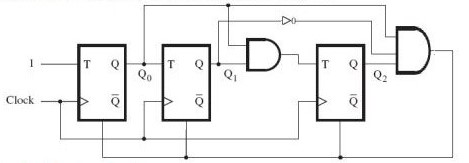
\includegraphics[width = 10cm]{images/contatore_mod_5.JPG}
    \caption{Contatore modulo 5}
\end{figure}

\section{Registri}
Un registro è un insieme di flip-flop che vengono utilizzati per memorizzare valori.

Possiamo effettuare due tipi di operazioni sui registri ovvero il \textbf{caricamento}, che riguarda la scrittura o input dei dati e lo \textbf{scaricamento} per la lettura o output dei dati.

\begin{center}
    \begin{tikzpicture}
        % x line
        \draw(0,0) -- (5,0);\draw(0,0) -- (0,1);
        \draw(0,1) -- (5,1);\draw(5,0) -- (5,1);
        \draw(1,0) -- (1,1);\draw(2,0) -- (2,1);
        \draw(4,0) -- (4,1);\draw (3,0.3) -- (3,0.3) node [above] {. . .};
        \draw (0.5,0.3) -- (0.5,0.3) node [above] {FF};
       \draw[->](0.5,0) -- (0.5,-0.5);\draw[->](0.5,1.5) -- (0.5,1);
    \end{tikzpicture}
\end{center}

Entrambe le operazioni possono essere effettuate in \textbf{serale} o \textbf{parallelo}.

\subsubsection{Registri SISO (Serial Input Serial Output)}

\begin{center}
    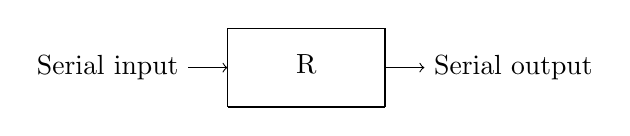
\begin{tikzpicture}
        % x line
        \draw(0,0) -- (2,0);\draw(0,0) -- (0,1);
        \draw(2,1) -- (2,0);\draw(0,1) -- (2,1);
        \draw (1,0.3) -- (1,0.3) node [above] {R};
       \draw[->](-0.5,0.5) -- (0,0.5);\draw[->](2,0.5) -- (2.5,0.5);
       \draw (-0.5,0.5) -- (-0.5,0.5) node [left] {Serial input};
       \draw (2.5,0.5) -- (2.5,0.5) node [right] {Serial output};
    \end{tikzpicture}
\end{center}

I registri SISO sono registri formati da una serie di FF di tipo D, sincronizzati tra di loro traminte clock.

\begin{figure}[H]
    \centering
    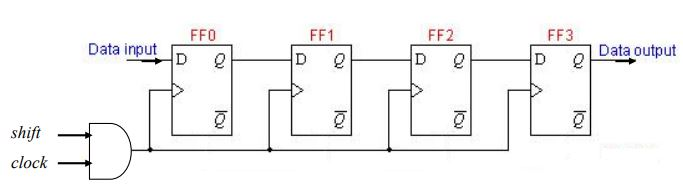
\includegraphics[width = 12cm]{images/siso.JPG}
    \caption{Registro SISO}
    \label{fig:SISO}
\end{figure}

I valori nei registri verranno inseriti in seriale tramite n impulsi di clock, dove n indica il numeri di flip-flop. Per caricare n bit, devo fare in modo che shift sia a 1 per n 
fronti d'onda discendenti del clock e che ad ogni fronte la linea dati entrante contenga il nuovo valore da memorizzare. Per scaricare il registro, bisogna settare shift per n cicli di clock e prelevare i bit dalla linea dati uscente.

\begin{example}
    Vogliamo caricare nel registro il valore 1101.
    
    Per la lettura/input si legge il valore nel registro, shiftando i valori verso la linea di uscita seriale, in n cicli di clock.
    \begin{center}
    \begin{tabular}{|c|c|}
         \hline Tempo & $y_3y_2y_1y_0$\\\hline\hline
         $t_0$ & 0000\\
         $t_1$ & 1000\\
         $t_2$ & 1100\\
         $t_3$ & 0110\\
         $t_4$ & 1011\\\hline
    \end{tabular}
    \end{center}
\end{example}

\subsubsection{Registro SIPO (Serial Input Parrallel Output)}
La costruzione di un registro SIPO è molto simile a quella del SISO, con la differenza che i valori di lettura/output vengono restituiti in parallelo.

\begin{center}
    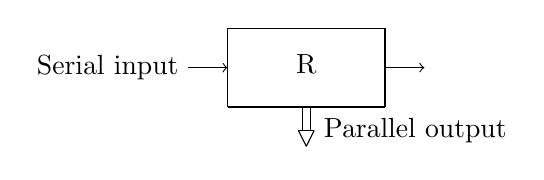
\begin{tikzpicture}
        % x line
        \draw(0,0) -- (2,0);\draw(0,0) -- (0,1);
        \draw(2,1) -- (2,0);\draw(0,1) -- (2,1);
        \draw (1,0.3) -- (1,0.3) node [above] {R};
       \draw[->](-0.5,0.5) -- (0,0.5);\draw[->](2,0.5) -- (2.5,0.5);
       \draw (-0.5,0.5) -- (-0.5,0.5) node [left] {Serial input};
       \draw (1.1,-0.3) -- (1.1,-0.3) node [right] {Parallel output};
       \draw(0.95,0) -- (0.95,-0.3);\draw(1.05,0) -- (1.05,-0.3);
       \draw(0.9,-0.3) -- (1.1,-0.3);\draw(0.9,-0.3) -- (1,-0.5);
       \draw(1,-0.5) -- (1.1,-0.3);
    \end{tikzpicture}
\end{center}

\begin{figure}[H]
    \centering
    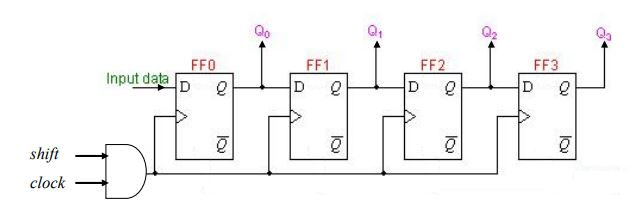
\includegraphics[width = 12cm]{images/sipo.JPG}
    \caption{Registro SIPO}
    \label{fig:SIPO}
\end{figure}

\subsubsection{Registro PISO (Parallel Input Serial Output)}
Nei registri con parallel input e serial output abbiamo lo stesso circuito del SISO con la differenza che le entrate: $x_0,x_1,x_{n-1}$ vengono inserite in parallelo e collegate ai flip-flop.

\begin{figure}[H]
    \centering
    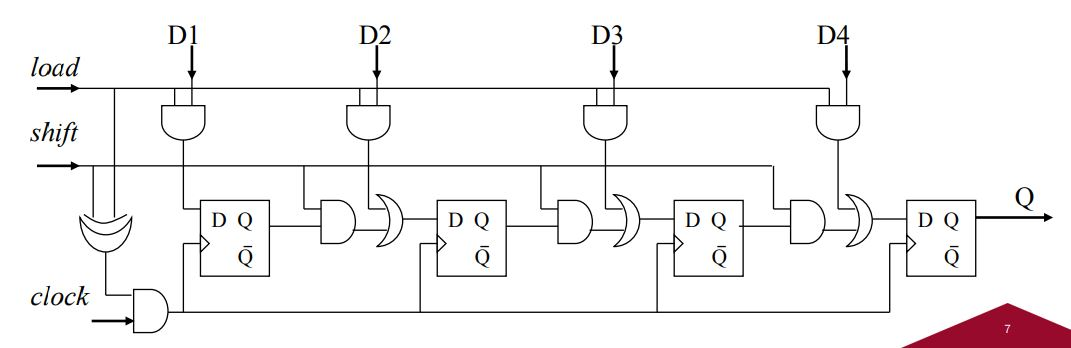
\includegraphics[width = 12cm]{images/piso.JPG}
    \caption{Registro PISO}
    \label{fig:SIPO}
\end{figure}

Il registro memorizza gli n input delle linee di dati quando il segnale load è a 1 e al momento di un fronte d'onda discendente del clock.
Il valore memorizzato viene scaricato quando shift vale 1 (in n fronti d'onda del clock). 

\textbf{N.B.} Load e shift non possono essere entrambe a 1 nello stesso istante.

\subsubsection{Registro PIPO (Parallel Input Parallel Output)}
Nei registri con parallel input e parallel output abbiamo lo stesso circuito del SIPO con la differenza che le entrate: $x_0,x_1,x_{n-1}$ vengono inserite in parallelo e collegate ai flip-flop.

\begin{figure}[H]
    \centering
    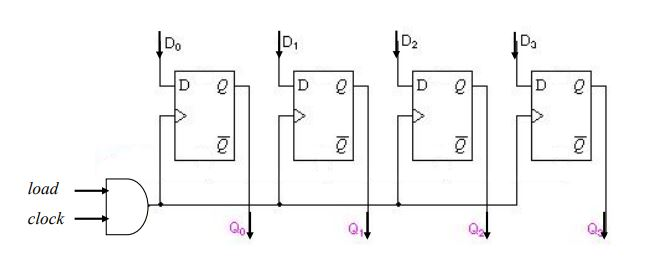
\includegraphics[width = 12cm]{images/pipo.JPG}
    \caption{Registro PIPO}
    \label{fig:SIPO}
\end{figure}

Il registro riceve in input n linee di dati; tali linee vengono memorizzate quando il segnale load è a 1 e al momento di un
fronte d'onda discendente del clock. Il valore memorizzato viene
riproposto in output dopo t. 

\subsubsection{Registri a rotazione destra}
Nel registro a rotazione a destra i valori vengono fatti ruotare all'interno dei flip-flop. Oltre al serial input trovaimo anche il control, ovvero un comando che può assumere valori 0 e 1 e in base a questi decidere se far ruotare i valori o far entrare il serial input.

\begin{figure}[H]
    \centering
    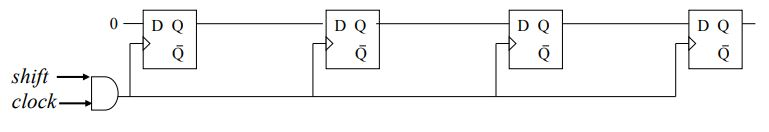
\includegraphics[width = 12cm]{images/right_shifter.JPG}
    \caption{Registro a rotazione a destra}
    \label{fig:r_rot_dx}
\end{figure}


\subsubsection{Registri a rotazione sinistra}
Il funzionamento dei registri a rotazione a sinistra è uguale a quelli con rotazione a destra con l'accortezza che il control e SI vengono spostati all'ultimo flip-flop e i valori vengono appunto shiftati a sinistra.
\begin{figure}[H]
    \centering
    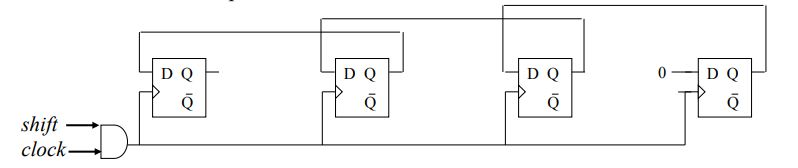
\includegraphics[width = 12cm]{images/left_shifter.JPG}
    \caption{Registro a rotazione a sinistra}
    \label{fig:r_rot_sx}
\end{figure}


\subsubsection{Registro universale}
\begin{center}
    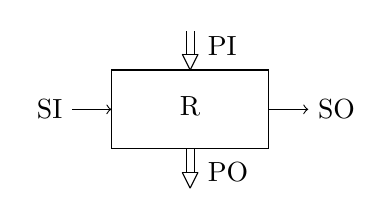
\begin{tikzpicture}
        % x line
        \draw(0,0) -- (2,0);\draw(0,0) -- (0,1);
        \draw(2,1) -- (2,0);\draw(0,1) -- (2,1);
        \draw (1,0.3) -- (1,0.3) node [above] {R};
       \draw[->](-0.5,0.5) -- (0,0.5);\draw[->](2,0.5) -- (2.5,0.5);
       \draw (-0.5,0.5) -- (-0.5,0.5) node [left] {SI};
       \draw (2.5,0.5) -- (2.5,0.5) node [right] {SO};
       \draw (1.1,-0.3) -- (1.1,-0.3) node [right] {PO};
       \draw (1.1,1.3) -- (1.1,1.3) node [right] {PI};
       \draw(0.95,0) -- (0.95,-0.3);\draw(1.05,0) -- (1.05,-0.3);
       \draw(0.9,-0.3) -- (1.1,-0.3);\draw(0.9,-0.3) -- (1,-0.5);
       \draw(1,-0.5) -- (1.1,-0.3);
       
       \draw(0.95,1.2) -- (0.95,1.5);\draw(1.05,1.2) -- (1.05,1.5);
       \draw(0.9,1.2) -- (1.1,1.2);\draw(0.9,1.2) -- (1,1);
       \draw(1,1) -- (1.1,1.2);
    \end{tikzpicture}
\end{center}

Nel registro universale abbiamo gli input inseriti in parallelo e seriale e lo stesso per gli output. Intoltre sono presenti le linee di LOAD: car parellelo, RS: right shift, LS: left shift e infine l'enable e il clock.

\begin{figure}[H]
    \centering
    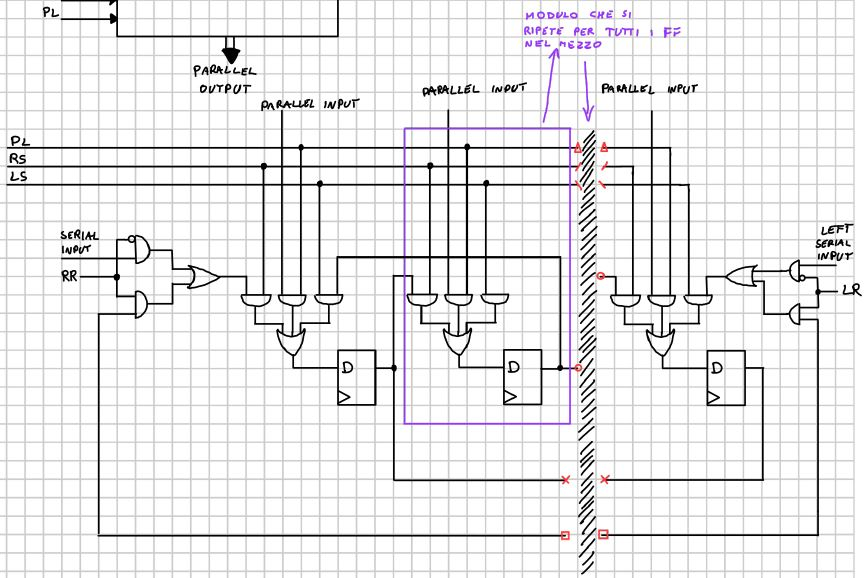
\includegraphics[width = 12cm]{images/registro_universale.JPG}
    \caption{Registro universale}
    \label{fig:r_unive}
\end{figure}


\section{Trasferimento tra registri}
Tramite il trasferimento tra registri vogliamo che il contenuto di un registro venga copiato in un registro destinazione.
Abbiamo per tanto quattro diverse modalità di trasferimento che dipendono dal numero di registri sorgente e destinazione:

\newcommand{\splitcell}[2][c]{%
  \begin{tabular}[c]{@{}c@{}}\strut#2\strut\end{tabular}%
}

\begin{table}[ht]
    \centering
    \begin{tabular}{|c||c|c|}
         \hline & 1 DESTINAZIONE & MOLTE DESTINAZIONI\\\hline\hline
         1 SORGENTE & \splitcell{Porte and\\Buffer tristate} & Decoder\\\hline
         MOLTE SORGENTI & Mux & \splitcell{Mesh (Mux)\\Bus}\\\hline
    \end{tabular}
    \caption{Modalità di trasferimento tra registri}
    \label{tab:mod_trasf_reg}
\end{table}

Vediamo ora in maniera schematica i vari casi:
\begin{figure}[ht]
    \centering
    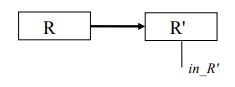
\includegraphics[width = 6cm]{images/uno_uno.JPG}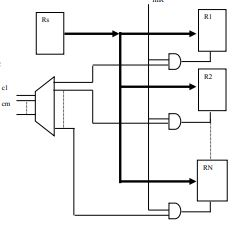
\includegraphics[width = 6cm]{images/uno_molti.JPG}
    \caption{Trasferimento con una sorgente e una/molte destinazioni}
\end{figure}
\begin{figure}[H]
    \centering
    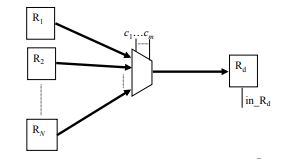
\includegraphics[width = 6cm]{images/molti_uno.JPG}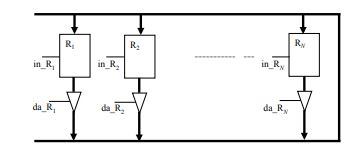
\includegraphics[width = 6cm]{images/molti_molti.JPG}
    \caption{Trasferimento con molte sorgenti e una/molte destinazioni}
\end{figure}

\subsubsection{Connessione uno a uno}
La connessione 1-A-1 è formata da un'insieme di flip-flop di tipo SR.
\begin{figure}[H]
    \centering
    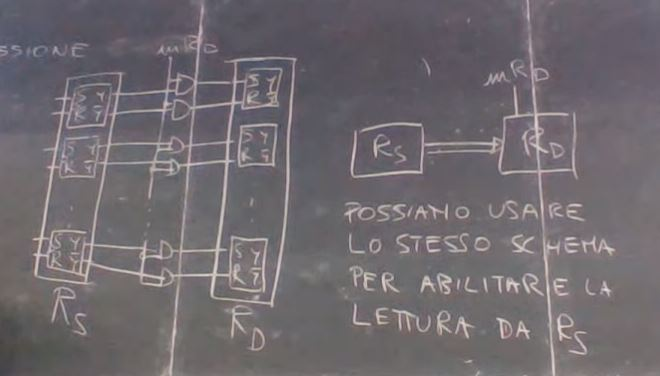
\includegraphics[width = 10cm]{images/1-a-1.JPG}
\end{figure}

Possiamo usare lo stesso schema per abilitare la lettura da $R_s$. In entrambe le rappresentazioni, possiamo usare buffer tristate al posto di porte and.

\subsubsection{Connessione uno a molti}
\begin{figure}[H]
    \centering
    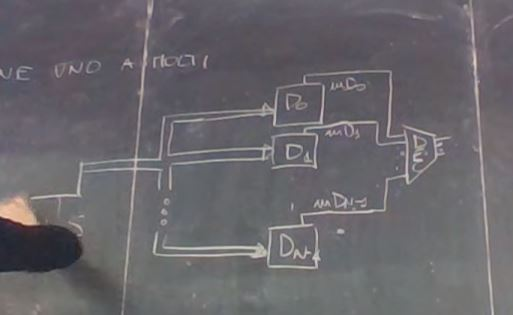
\includegraphics[width = 10cm]{images/1-a-1.1.JPG}
\end{figure}

\subsubsection{Connessione molti a uno}
\begin{figure}[H]
    \centering
    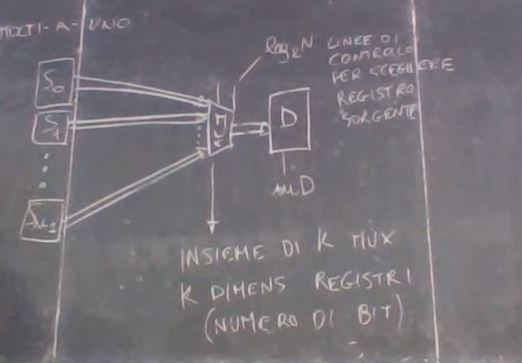
\includegraphics[width = 10cm]{images/1-a-molti.JPG}
\end{figure}

Nelle connessioni molti-a-uno possiamo trovare due costruzioni differenti. Una mesh che si utilizza quando abbiamo registri vicini tra di loro o un bus per quelli lontani.


\subsubsection{Connessione molti a molti}
Anche in questo caso abbiamo un mesh:
\begin{figure}[H]
    \centering
    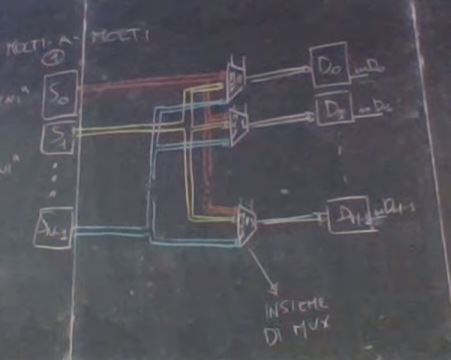
\includegraphics[height = 5cm]{images/molti-a-molti.JPG}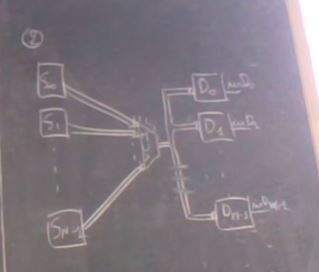
\includegraphics[height = 5cm]{images/molti-a-molti.1.JPG}
\end{figure}

O un bus

\begin{figure}[H]
    \centering
    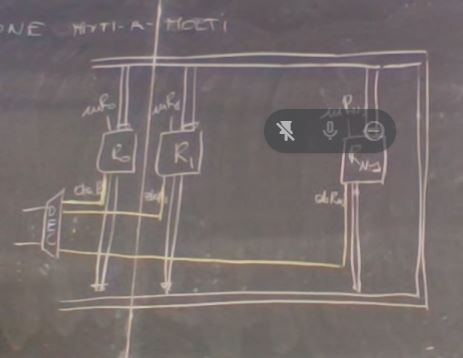
\includegraphics[width = 10cm]{images/molti-a-molti-2.JPG}
\end{figure}

\subsection{Progettare uno schema di connessione tra registri}
Per progettare uno schema di connessione tra registri dobbiamo:
\begin{itemize}
    \item Individuare lo schema per trovare le informazioni;
    \item Progettare lo schema dei segnali di controllo (come parità(LSB), pos/neg(MSB), multipli di $2^k$(LSB));
    \item Aggiungere i moduli standard (MUX, DEC, ADDER, COMPARATORI).
\end{itemize}

Per approfondire vedi Esercizio \ref{ex_coll_reg1}.

\newpage
\section{Esercizi svolti}
\begin{exercise}
     Sia dato un UP-counter sincrono modulo 4. Si effettui l’analisi (fino all’automa minimo) del seguente circuito sequenziale, inizialmente impostato a y0=1 e y1=y2=0.
     \begin{figure}[ht]
         \centering
         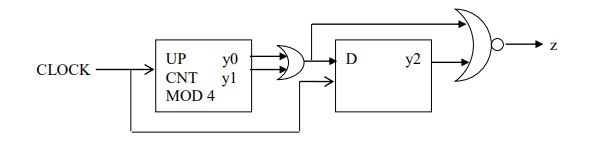
\includegraphics[width = 11cm]{images/registri_es_1.JPG}
         \caption{Circuito da analizzare}
         \label{fig:registri_es_1}
     \end{figure}
     
     \begin{enumerate}
         \item Calcolo le espressioni booleane delle funzioni di eccitazione e delle uscite:
         \begin{equation*}
             D = y_1+y_0\hspace{1cm}z=\overline{(y_1+y_0)+y_2}=\overline{y_2}\overline{y_1}\overline{y_0}
         \end{equation*}
         
         \item Scrivo la tavola degli stati futuri. Guardando il nostro circuito \ref{fig:registri_es_1}, possiamo compilare lo stato futuro $Y_2$ tramite $y_2$ e il FF D, mentre gli stati $y_1$ e $y_0$ guardando lo stato successivo perchè ci troviamo in un counter.
         
         \begin{table}[ht]
            \centering
            \begin{tabular}{|c|c|c|c|}
                 \hline $y_2y_1y_0$ & $D$ & $z$ & $Y_2Y_1Y_0$\\\hline\hline
                 000 & 0 & 1 & 001\\
                 001 & 1 & 0 & 110\\
                 010 & 1 & 0 & 111\\
                 011 & 1 & 0 & 100\\\hline
                 100 & 0 & 0 & 011\\
                 101 & 1 & 0 & 110\\
                 110 & 1 & 0 & 111\\
                 111 & 1 & 0 & 100\\\hline
            \end{tabular}
            \caption{Tavola degli stati futuri}
    \end{table}
         
         \item Scriviamo gli stati $Q_n$ come: $Q_0=000$, $Q_1=001$, ... $Q_7=111$ e stendiamo la tavola dell'automa:
         
         \begin{table}[ht]
             \centering
             \begin{tabular}{|c|c|}
                  \hline Stato attuale & Stato futuro$\backslash$uscita\\\hline\hline
                  $Q_0$ & \diagbox[width=1.5cm]{$Q_1$}{1}\\\hline
                  $Q_1$ & \diagbox[width=1.5cm]{$Q_6$}{0}\\\hline
                  $Q_2$ & \diagbox[width=1.5cm]{$Q_7$}{0}\\\hline
                  $Q_3$ & \diagbox[width=1.5cm]{$Q_4$}{0}\\\hline
                  $Q_4$ & \diagbox[width=1.5cm]{$Q_1$}{0}\\\hline
                  $Q_5$ & \diagbox[width=1.5cm]{$Q_6$}{0}\\\hline
                  $Q_6$ & \diagbox[width=1.5cm]{$Q_7$}{0}\\\hline
                  $Q_7$ & \diagbox[width=1.5cm]{$Q_4$}{0}\\\hline
             \end{tabular}
             \caption{Tavola dell'automa}
         \end{table}
         
         Notiamo come gli stati $Q_2$ e $Q_6$, $Q_3$ e $Q_7$, $Q_1$ e $Q_5$ sono equivalenti. Possiamo direttamente semplificare l'automa scrivendo:
         \begin{equation*}
             Q'_2=\{Q_2,Q_6\}\hspace{1cm}Q'_3=\{Q_3,Q_7\}\hspace{1cm}Q'_1=\{Q_1,Q_5\}
         \end{equation*}
         
         \item Disegnamo ora il diagramma dell'automa sapendo, dalla traccia, che lo stato iniziale è 001 ovvero $Q_1$:
         \begin{figure}[H]
             \centering
             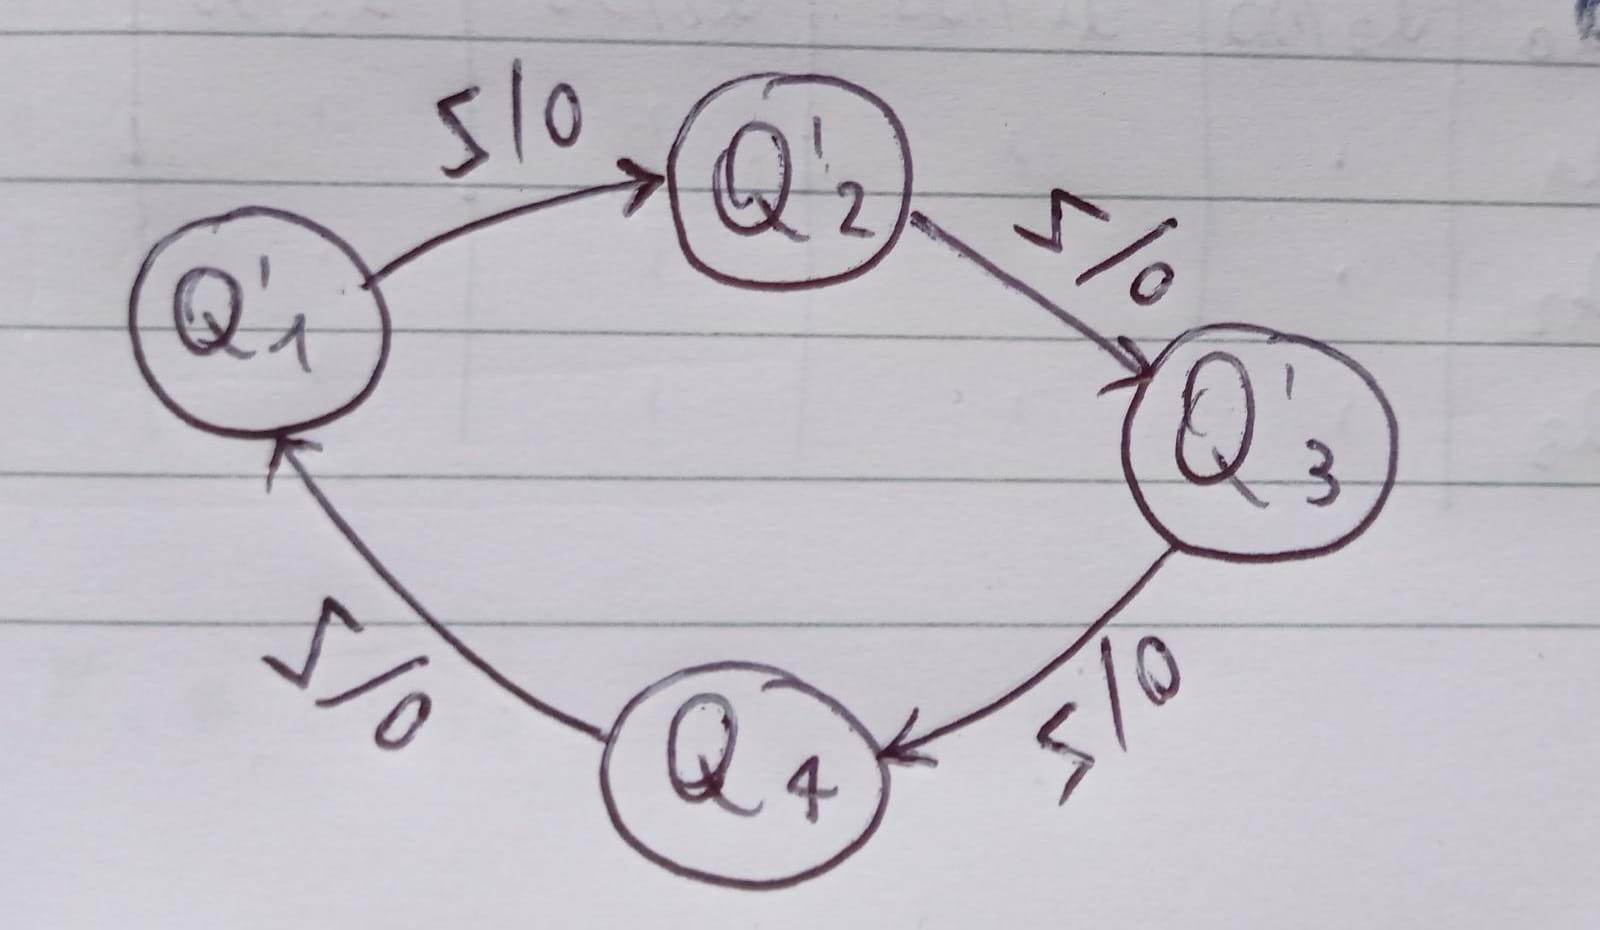
\includegraphics[width = 7cm]{images/registri_es1_diagautom.jpeg}
             \caption{Diagramma dell'automa}
         \end{figure}
     \end{enumerate}
\end{exercise}

\begin{exercise}\label{ex_coll_reg1}
     Considerate un insieme di 10 registri $R_i$ (con i = 0, ..., 9) interconnessi tramite bus. Progettare i seguenti trasferimenti:
     \begin{itemize}
         \item Se $R_0$ è pari $R_8$ viene trasferito nei registri $R_j$ con j = 4, ..., 7, altrimenti $R_7$ viene trasferito nei registri $R_k$ con k = 1, ..., 3.
         \item I trasferimenti sono abilitati se $R_9$ è multiplo di 4.
         
         \begin{figure}[H]
             \centering
             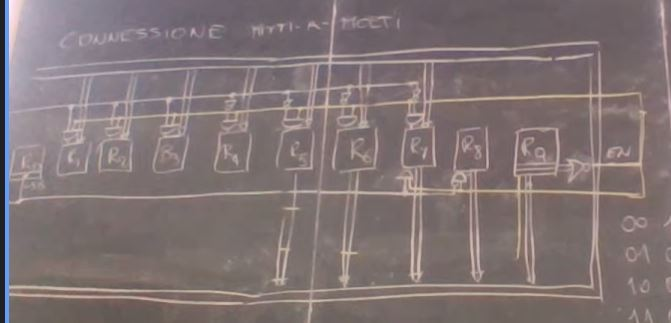
\includegraphics[width = 12cm]{images/connessione-es.JPG}
             \caption{Registro risultante}
         \end{figure}
     \end{itemize}
\end{exercise}

\begin{exercise}
     Si progetti la rete di interconnessione tale che:
\begin{itemize}
    \item $R_3$ viene trasferito in $R_0$ se $R_1$ e $R_2$ sono discordi, in $R_1$ altrimenti;
    \item in $R_3$ viene trasferita la differenza tra $R_1$ e $R_2$ se il contenuto di R0 non è multiplo di 4, la somma tra $R_1$ e $R_2$ altrimenti;
\end{itemize}

Tutti i trasferimenti sono abilitati se $R_0$ e $R_1$ sono entrambi pari.

\begin{figure}[H]
    \centering
    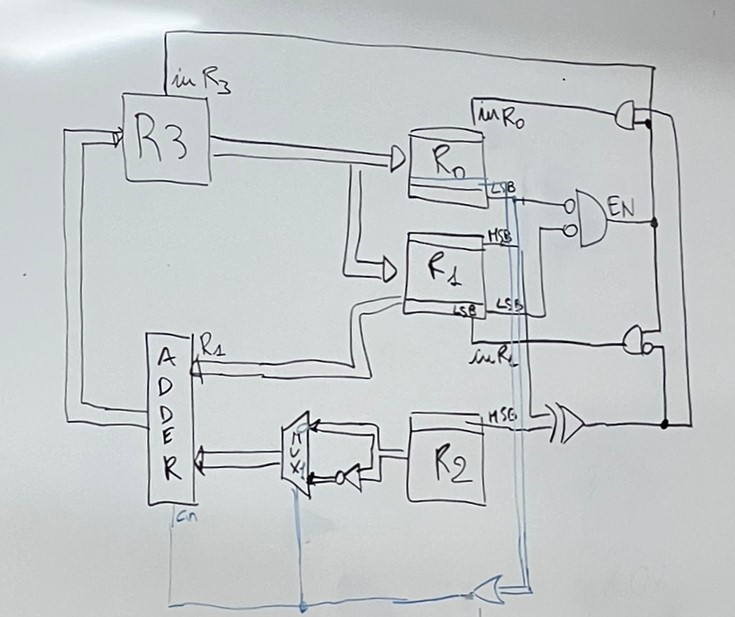
\includegraphics[width = 9cm]{images/es_2_registri.jpeg}
    \caption{Registro risultante}
\end{figure}
\end{exercise}
